\documentclass[12pt, letterpaper]{article}
\usepackage{graphicx}
\usepackage{hyperref}
\usepackage{amssymb}
\usepackage{amsmath}
\usepackage{float}
\usepackage{mathtools}
\usepackage{enumitem}
\usepackage[margin=1in]{geometry}
\usepackage[figurename=Figura]{caption}

\title{%
  Situación Problema: Análisis de Audio usando Fourier \\
  \large F1009: Análisis de métodos matemáticos para la física}

\begin{document}

\maketitle

\begin{tabular}{ccc}
Juan Pablo Guerrero Escudero & Romina Nájera Fuentes & Juan Braulio Olivares Rodríguez
\end{tabular}

\section*{Introducción}

\section*{Teoría}

Conceptos de física relevantes:
\begin{enumerate}
    \item Ondas de sonido\\
    De acuerdo a Young y Freedman \cite{university-physics}, El sonido se define como una onda 
    longitudinal en un medio, principalmente aire, pero puede ser otros como otros gases, líquidos o sólidos. Las 
    ondas de sonido más simple son ondas sinusoidales con una frecuencia, amplitud y longitud definida. 
    \cite{university-physics}. El ser humano es capaz de escuchar ondas en el rango de 20 a 20,000 Hz, con 
    frecuencias por encima del rango (ultrasónicas) o debajo del rango (infrasónicas) fuera del rango de escucha humano. 
    De acuerdo a Hwaitat \cite{frequencies-wave-sound-pso}, las ondas de sonido son peturbancias propagadas por un medio el cuál 
    no se ve afectado, y éstas ondas pueden ser ya sea longitudinales, o transversales. Para una onda 
    de tipo longitudinal, el medio vibra en ángulos rectos al movimiento de la onda, y en el caso de ondas longitudinales, 
    el medio vibra en la misma dirección que el movimiento.En la Figura \ref*{Ondas Longitudinales} se observa gráficamente lo discutido. 
    \begin{figure}[H]
      \centering
      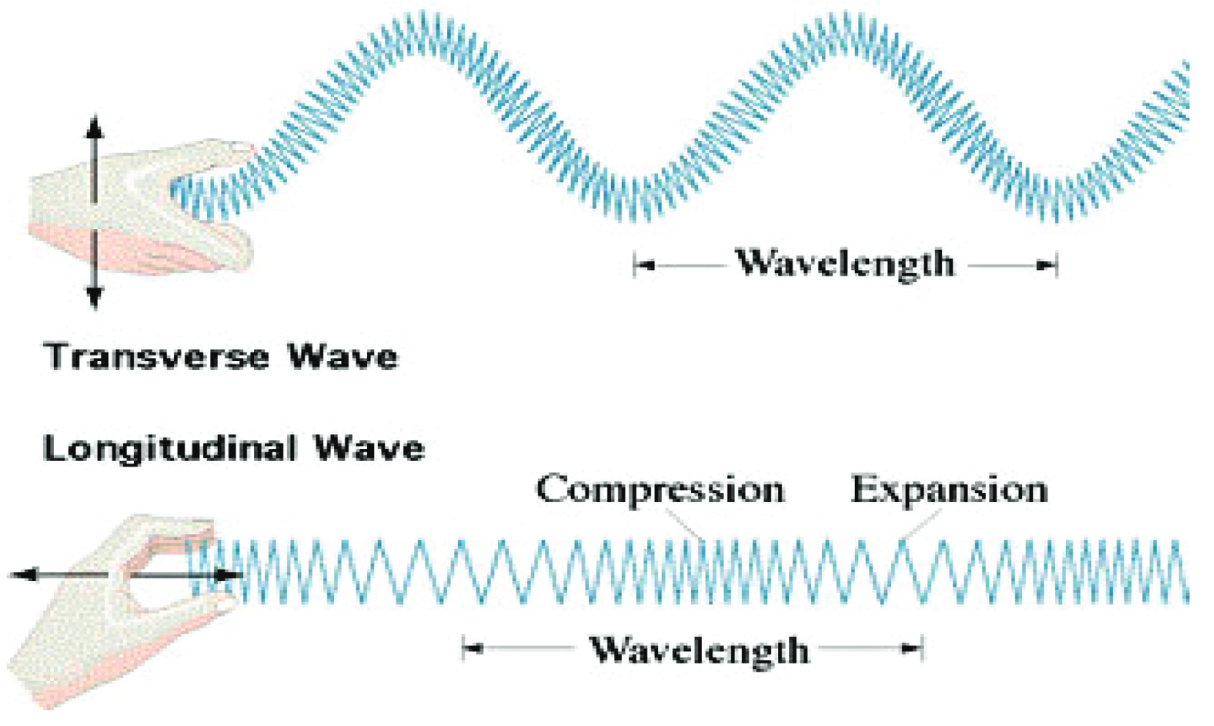
\includegraphics[height = 4cm]{ondas_longitudinales_transversales.png}
      \caption{Ondas longitudinales y transversales}
      \label{Ondas Longitudinales}
    \end{figure}
    Los parámetros de cualquier onda constituyen la amplitud, la frecuencia 
    y la longitud, mencionados anteriormente. La amplitud puede ser definida como la "altura" 
    de la onda, la frecuencia se define como los ciclos por segundo, y la longitud se define como la distancia 
    entre un pico de onda y otro. Para una vista gráfica, vea la Figura \ref*{parametros-ondas}. Generalmente, sucede que 
    cuando dos partículas están en movimiento en el mismo medio, ocurre interferencia. Ésto significa que 
    las amplitudes de onda son sumadas algebraicamente, y se siguen moviendo por el medio sin distracciones. En el mundo real, 
    la interferencia de ondas crea patrones complejo, y puede ser muy difícil de analizar.  
    \begin{figure}[H]
      \centering
      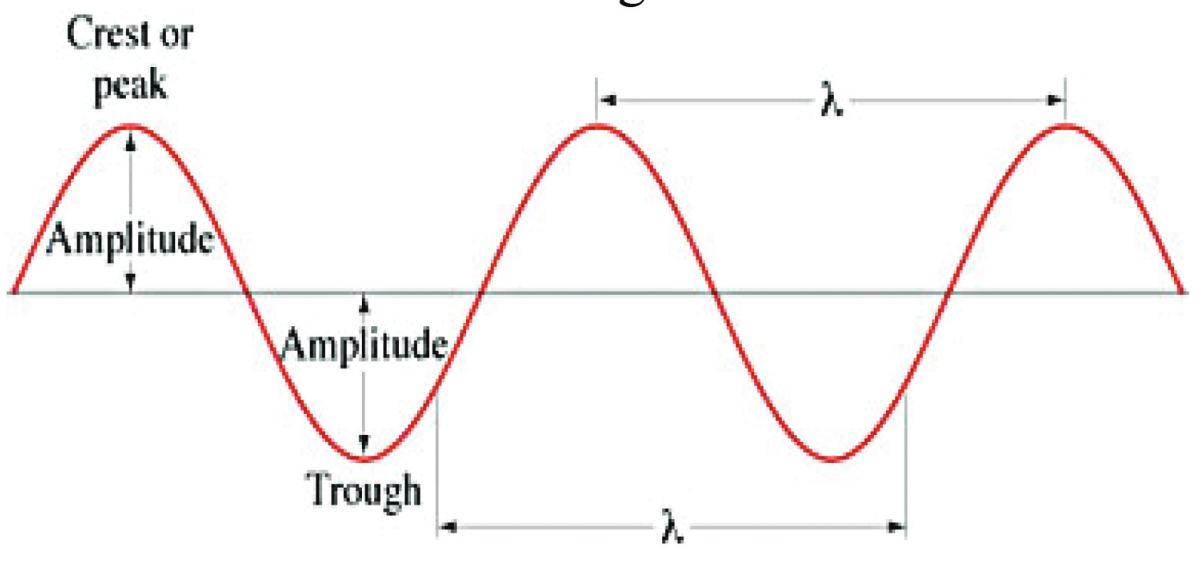
\includegraphics[height = 4cm]{parametros-ondas.png}
      \caption{Parámetros de las ondas de sonido}
      \label{parametros-ondas}
    \end{figure}
    \item Frecuencias de audio/sonido. \\
    Como se definió anteriormente, la frecuencia de una onda es, de acuerdo a [1], como el número de repeticiones 
    de una función periódica durante una unidad de variación en la variable independiente. En otras palabras, es el número de 
    ocurrencias de un evento repetitivo por unidad de tiempo. 
    \item Sonidos armónicos
    \item Beats
\end{enumerate}

\noindent Análisis matemático + fundamentos:
\begin{enumerate}
    \item Análisis espectral de canciones
    \item Transformada de Fourier
    \item Identificación de reggaeton/instrumental
\end{enumerate}



\section*{Resultados}

\section*{Conclusiones}

\section*{Referencias}
\begin{thebibliography}{9}
  \bibitem{university-physics}
  H. D. Young and Roger A. Freedman, \emph{University Physics with Modern Physics}, 
Addison-Wesley, San Francisco, 2012. %%Para citar \cite{university-physics}

  \bibitem{frequencies-wave-sound-pso}
Al Hwaitat et Al, Journal of Experimental \&\ Theoretical Artificial Intelligence, 
2022, 34, 749-780
  \end{thebibliography}
\end{document}
